\section{Solution of Initial Value Problems}

\noindent
\boxit{Laplace Transforms of Derivatives}

\noindent
In the rest of this chapter we'll use the Laplace transform to solve initial value problems for
constant coefficient second order equations. To do this, we must know how the Laplace transform of
$f'$ is related to the Laplace transform of $f$. The next theorem answers this question.

\begin{theorem}
  \color{blue}
  \label{thmtype:8.3.1} Suppose $f$ is continuous on $[0,\infty)$ and of exponential order $s_{0}$,
  and $f'$ is piecewise continuous on $[0,\infty)$. Then $f$ and $f'$ have Laplace transforms for
  $s>s_{0}$, and
  \begin{equation}
    \label{eq:8.3.1}{\cal L}(f')=s{\cal L}(f)-f(0).
  \end{equation}
\end{theorem}

\proof

We know from Theorem~8.1.6 that ${\cal L}(f)$ is defined for $s>s_{0}$. We first consider the case
where $f'$ is continuous on $[0,\infty)$. Integration by parts yields
\begin{equation}
  \label{eq:8.3.2}
  \begin{array}{ccl}
    \dst\int^{T}_{0}e^{-st}f'(t)\,dt & = & \dst e^{-st}f(t)\Big|^{T}_{0}+s \dst\int^{T}_{0}e^{-st}f(t)\,dt \\
                                     & = & \dst e^{-sT}f(T)-f(0)+s\int^{T}_{0}e^{-st}f(t)\,dt
  \end{array}
\end{equation}
for any $T>0$. Since $f$ is of exponential order $s_{0}$, $\lim_{T\to\infty}e^{-sT}f(T)=0$ and the
last integral in \eqref{eq:8.3.2} converges as $T\to\infty$ if $s>s_{0}$. Therefore
\begin{eqnarray*}
  \int^{\infty}_{0}e^{-st}f'(t)\,dt & = & -f(0)+s\int^{\infty}_{0}e^{-st}f(t)\,dt \\
                                    & = & -f(0)+s{\cal L}(f),
\end{eqnarray*}
which proves \eqref{eq:8.3.1}. Now suppose $T>0$ and $f'$ is only piecewise continuous on $[0,T]$,
with discontinuities at $t_{1}<t_{2}<\cdots<t_{n-1}$. For convenience, let $t_{0}=0$ and $t_{n}=T$.
Integrating by parts yields
\begin{eqnarray*}
  \int^{t_{i}}_{t_{i-1}}e^{-st}f'(t)\,dt & = & e^{-st}f(t)\Big|^{t_{i}}_{t_{i-1}}+s\int^{t_{i}}_{t_{i-1}}e^{-st}f(t)\,dt \\
                                         & = & e^{-st_{i}}f(t_{i})-e^{-st_{i-1}}f(t_{i-1})+s\int^{t_{i}}_{t_{i-1}}e^{-st}f(t)\,dt.
\end{eqnarray*}
Summing both sides of this equation from $i=1$ to $n$ and noting that
\[
  \left(e^{-st_{1}}f(t_{1})-e^{-st_{0}}f(t_{0})\right)+\left(e^{-st_{2}}f(t_{2})-e^{-st_{1}}f(t_{1})\right) +\cdots+\left(e^{-st_{N}}f(t_{N})-e^{-st_{N-1}}f(t_{N-1})\right)
\]
\[
  =e^{-st_{N}}f(t_{N})-e^{-st_{0}}f(t_{0})=e^{-sT}f(T)-f(0)
\]
yields \eqref{eq:8.3.2}, so \eqref{eq:8.3.1} follows as before.

\begin{example}
  \label{example:8.3.1}\rm In Example~\ref{example:8.1.4} we saw that
  \[
    {\cal L}(\cos\omega t)=\frac{s}{s^{2}+\omega^{2}}.
  \]
  Applying \eqref{eq:8.3.1} with $f(t)=\cos\omega t$ shows that
  \[
    {\cal L}(-\omega\sin\omega t)=s\frac{s}{s^{2}+\omega^{2}}-1=- \frac{\omega^{2}}{s^{2}+\omega^{2}}.
  \]
  Therefore
  \[
    {\cal L}(\sin\omega t)=\frac{\omega}{s^{2}+\omega^{2}},
  \]
  which agrees with the corresponding result obtained in \ref{example:8.1.4}. \bbox
\end{example}

In Section~2.1 we showed that the solution of the initial value problem
\begin{equation}
  \label{eq:8.3.3}y'=ay,\quad y(0)=y_{0},
\end{equation}
is $y=y_{0}e^{at}$. We'll now obtain this result by using the Laplace transform.

Let $Y(s)={\cal L}(y)$ be the Laplace transform of the unknown solution of \eqref{eq:8.3.3}. Taking
Laplace transforms of both sides of \eqref{eq:8.3.3} yields
\[
  {\cal L}(y')={\cal L}(ay),
\]
which, by Theorem~\ref{thmtype:8.3.1}, can be rewritten as
\[
  s{\cal L}(y)-y(0)=a{\cal L}(y),
\]
or
\[
  sY(s)-y_{0}=aY(s).
\]
Solving for $Y(s)$ yields
\[
  Y(s)=\frac{y_{0}}{s-a},
\]
so
\[
  y={\cal L}^{-1}(Y(s))={\cal L}^{-1}\left(\frac{y_{0}}{s-a}\right)=y_{0}{\cal L}^{-1}\left(\frac{1}{s-a}\right)=y_{0}e^{at},
\]
which agrees with the known result.

We need the next theorem to solve second order differential equations using the Laplace transform.

\begin{theorem}
  \color{blue}
  \label{thmtype:8.3.2} Suppose $f$ and $f'$ are continuous on $[0,\infty)$ and of exponential order
  $s_{0}$, and that $f''$ is piecewise continuous on $[0,\infty)$. Then $f$, $f'$, and $f''$ have
  Laplace transforms for $s >s_{0}$,
  \begin{equation}
    \label{eq:8.3.4}{\cal L}(f')=s{\cal L}(f)-f(0),
  \end{equation}
  and
  \begin{equation}
    \label{eq:8.3.5}{\cal L}(f'')=s^{2}{\cal L}(f)-f'(0)-sf(0).
  \end{equation}
\end{theorem}

\proof Theorem~\ref{thmtype:8.3.1} implies that ${\cal L}(f')$ exists and satisfies \eqref{eq:8.3.4}
for $s>s_{0}$. To prove that ${\cal L}(f'')$ exists and satisfies \eqref{eq:8.3.5} for $s>s_{0}$, we
first apply Theorem~\ref{thmtype:8.3.1} to $g=f'$. Since $g$ satisfies the hypotheses of
Theorem~\ref{thmtype:8.3.1}, we conclude that ${\cal L}(g')$ is defined and satisfies
\[
  {\cal L}(g')=s{\cal L}(g)-g(0)
\]
for $s>s_{0}$. However, since $g'=f''$, this can be rewritten as
\[
  {\cal L}(f'')=s{\cal L}(f')-f'(0).
\]
Substituting \eqref{eq:8.3.4} into this yields \eqref{eq:8.3.5}.

\boxit{Solving Second Order Equations with the Laplace Transform}

\noindent
We'll now use the Laplace transform to solve initial value problems for second order equations.

\begin{example}
  \label{example:8.3.2}\rm Use the Laplace transform to solve the initial value problem
  \begin{equation}
    \label{eq:8.3.6}y''-6y'+5y=3e^{2t},\quad y(0)=2,\quad y'(0)=3.
  \end{equation}
\end{example}

\solution Taking Laplace transforms of both sides of the differential equation in \eqref{eq:8.3.6}
yields
\[
  {\cal L}(y''-6y'+5y)={\cal L}\left(3e^{2t}\right)=\frac{3}{s-2},
\]
which we rewrite as
\begin{equation}
  \label{eq:8.3.7}{\cal L}(y'')-6{\cal L}(y')+5{\cal L}(y)=\frac{3}{s-2}.
\end{equation}
Now denote ${\cal L}(y)=Y(s)$. Theorem~\ref{thmtype:8.3.2} and the initial conditions in
\eqref{eq:8.3.6} imply that
\[
  {\cal L}(y')=sY(s)-y(0)=sY(s)-2
\]
and
\[
  {\cal L}(y'')=s^{2}Y(s)-y'(0)-sy(0)=s^{2}Y(s)-3-2s.
\]
Substituting from the last two equations into \eqref{eq:8.3.7} yields
\[
  \left(s^{2}Y(s)-3-2s\right)-6\left(sY(s)-2\right)+5Y(s)=\frac{3}{s-2}.
\]
Therefore
\begin{equation}
  \label{eq:8.3.8}(s^{2}-6s+5)Y(s)=\frac{3}{s-2}+(3+2s)+6(-2),
\end{equation}
so
\[
  (s-5)(s-1)Y(s)=\frac{3+(s-2)(2s-9)}{s-2},
\]
and
\[
  Y(s)=\frac{3+(s-2)(2s-9)}{(s-2)(s-5)(s-1)}.
\]
Heaviside's method yields the partial fraction expansion
\[
  Y(s)=-\frac{1}{s-2}+\frac{1}{2}\frac{1}{s-5}+\frac{5}{2}\frac{1}{s-1},
\]
and taking the inverse transform of this yields
\[
  y=-e^{2t}+\frac{1}{2}e^{5t}+\frac{5}{2}e^{t}
\]
as the solution of \eqref{eq:8.3.6}.\bbox

It isn't necessary to write all the steps that we used to obtain \eqref{eq:8.3.8}. To see how to
avoid this, let's apply the method of Example~\ref{example:8.3.2} to the general initial value
problem
\begin{equation}
  \label{eq:8.3.9}ay''+by'+cy=f(t),\quad y(0)=k_{0},\quad y'(0)=k_{1}.
\end{equation}

Taking Laplace transforms of both sides of the differential equation in \eqref{eq:8.3.9} yields
\begin{equation}
  \label{eq:8.3.10}a{\cal L}(y'')+b{\cal L}(y')+c{\cal L}(y)=F(s).
\end{equation}
Now let $Y(s)={\cal L}(y)$. Theorem~\ref{thmtype:8.3.2} and the initial conditions in
\eqref{eq:8.3.9} imply that
\[
  {\cal L}(y')=sY(s)-k_{0}\mbox{\quad and \quad}{\cal L}(y'')=s^{2}Y(s)-k_{1}-k_{0}s.
\]
Substituting these into \eqref{eq:8.3.10} yields
\begin{equation}
  \label{eq:8.3.11}a\left(s^{2}Y(s)-k_{1}-k_{0}s\right)+b\left(sY(s)-k_{0}\right)+cY(s)=F(s).
\end{equation}
The coefficient of $Y(s)$ on the left is the characteristic polynomial
\[
  p(s)=as^{2}+bs+c
\]
of the complementary equation for \eqref{eq:8.3.9}. Using this and moving the terms involving
$k_{0}$ and $k_{1}$ to the right side of \eqref{eq:8.3.11} yields
\begin{equation}
  \label{eq:8.3.12}p(s)Y(s)=F(s)+a(k_{1}+k_{0}s)+bk_{0}.
\end{equation}
This equation corresponds to \eqref{eq:8.3.8} of Example~\ref{example:8.3.2}. Having established the
form of this equation in the general case, it is preferable to go directly from the initial value
problem to this equation. You may find it easier to remember \eqref{eq:8.3.12} rewritten as
\begin{equation}
  \label{eq:8.3.13}p(s)Y(s)=F(s)+a\left(y'(0)+sy(0)\right)+by(0).
\end{equation}

\begin{example}
  \label{example:8.3.3}\rm Use the Laplace transform to solve the initial value problem
  \begin{equation}
    \label{eq:8.3.14}2y''+3y'+y=8e^{-2t},\quad y(0)=-4,\;y'(0)=2.
  \end{equation}
\end{example}
\solution The characteristic polynomial is
\[
  p(s)=2s^{2}+3s+1=(2s+1)(s+1)
\]
and
\[
  F(s)={\cal L}(8e^{-2t})=\frac{8}{s+2},
\]
so \eqref{eq:8.3.13} becomes
\[
  (2s+1)(s+1)Y(s)=\frac{8}{s+2}+2(2-4s)+3(-4).
\]
Solving for $Y(s)$ yields
\[
  Y(s)=\frac{4\left(1-(s+2)(s+1)\right)}{(s+1/2)(s+1)(s+2)}.
\]
Heaviside's method yields the partial fraction expansion
\[
  Y(s)=\frac{4}{3}\frac{1}{s+1/2}-\frac{8}{s+1}+\frac{8}{3}\frac{1}{s+2},
\]
so the solution of \eqref{eq:8.3.14} is
\[
  y={\cal L}^{-1}(Y(s))=\frac{4}{3}e^{-t/2}-8e^{-t}+\frac{8}{3}e^{-2t}
\]
(Figure~\ref{figure:8.3.1}).

\begin{figure}[htbp]
  \color{blue}
  \begin{minipage}[b]{0.5\linewidth}
    \centering
    \scalebox{.65}{
    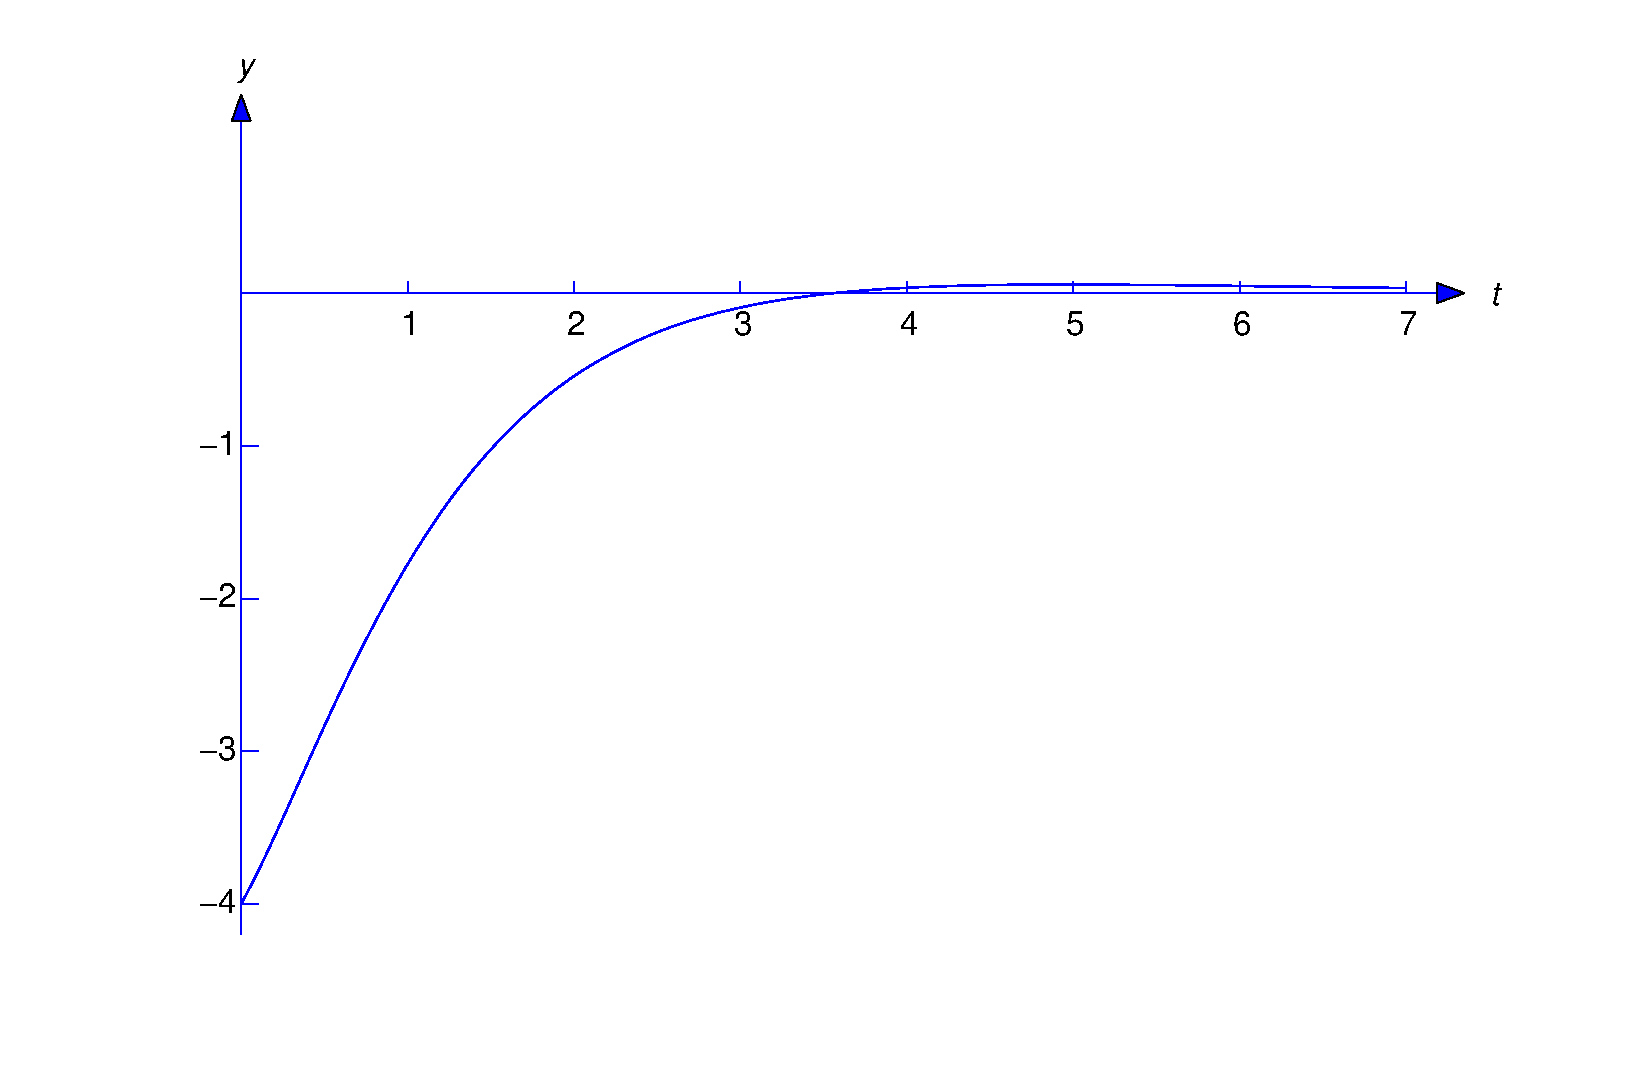
\includegraphics[bb=-78 148 689 643, width=5.67in, height=3.66in, keepaspectratio]{fig080301}}
    \caption{$y=\dst{\frac{4}{3}e^{-t/2}-8e^{-t}+\frac{8}{3}e^{-2t}}$}
    \label{figure:8.3.1}
  \end{minipage}
  \begin{minipage}[b]{0.5\linewidth}
    \centering
    \scalebox{.65}{
    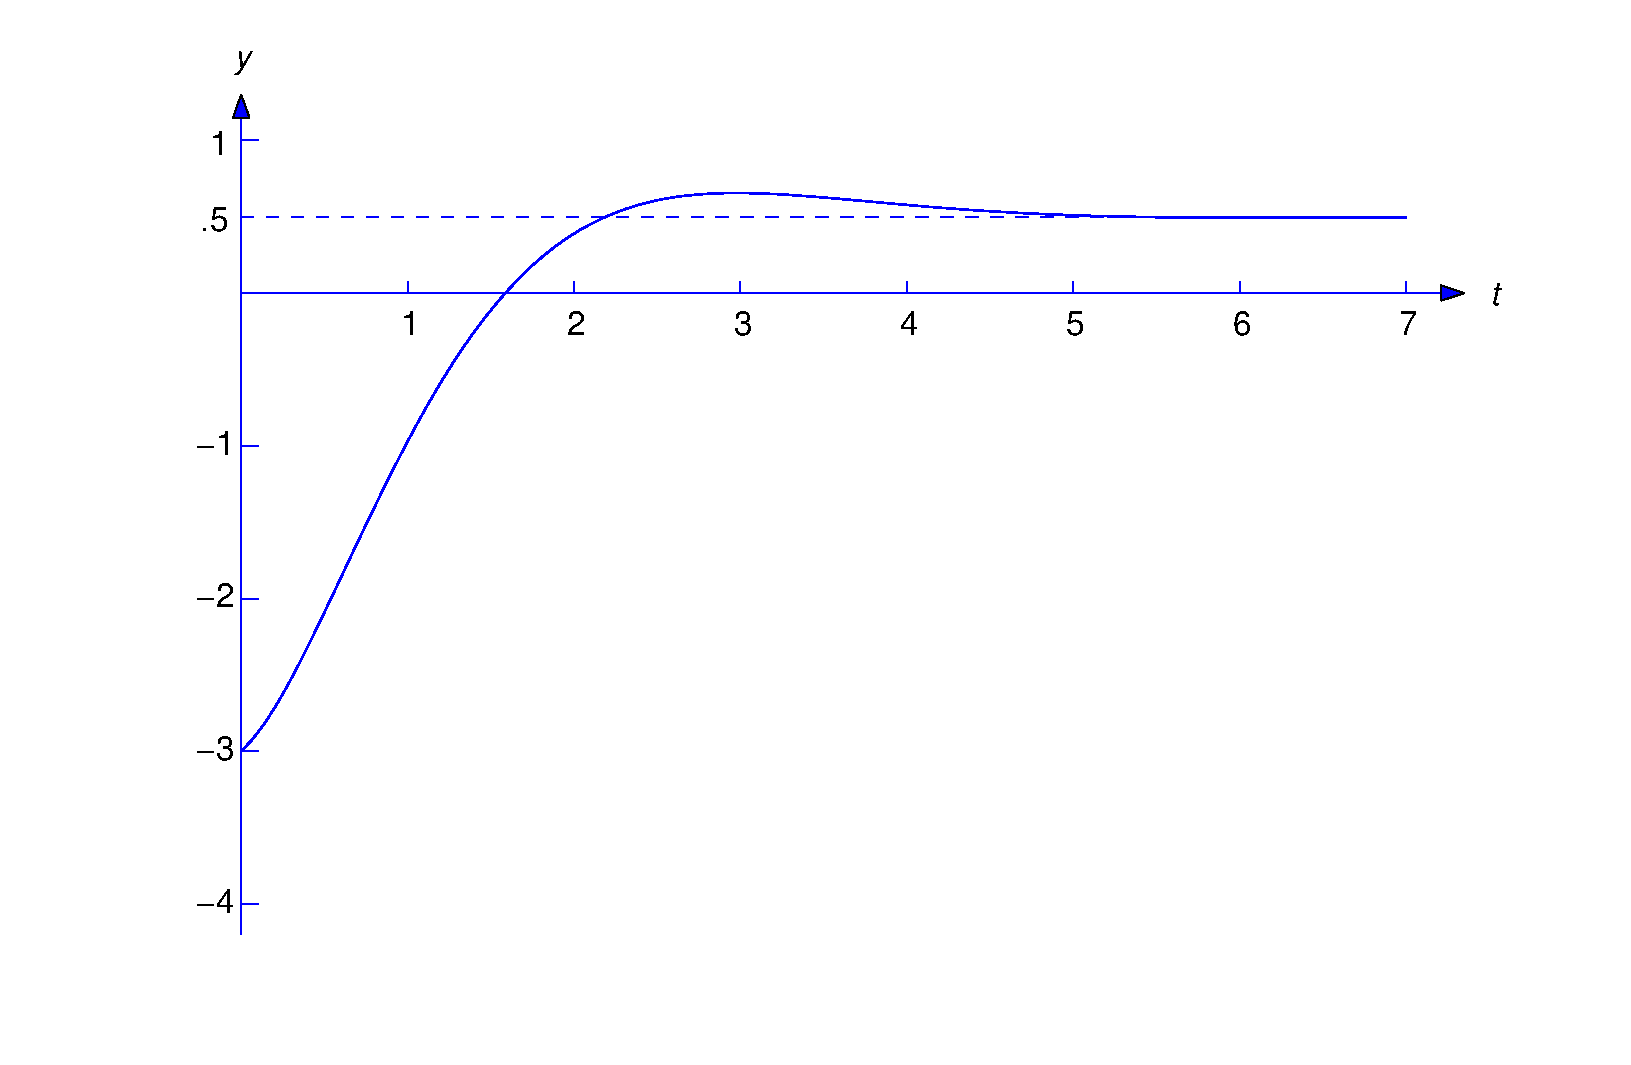
\includegraphics[bb=-78 148 689 643, width=5.67in, height=3.66in, keepaspectratio]{fig080302}}
    \caption{$y=\dst{\frac{1}{2}-\frac{7}{2}e^{-t}\cos t-\frac{5}{2}e^{-t}\sin t}$}
    \label{figure:8.3.2}
  \end{minipage}
\end{figure}

\begin{example}
  \label{example:8.3.4}\rm Solve the initial value problem
  \begin{equation}
    \label{eq:8.3.15}y''+2y'+2y=1,\quad y(0)=-3,\;y'(0)=1.
  \end{equation}
\end{example}

\solution The characteristic polynomial is
\[
  p(s)=s^{2}+2s+2=(s+1)^{2}+1
\]
and
\[
  F(s)={\cal L}(1)=\frac{1}{s},
\]
so \eqref{eq:8.3.13} becomes
\[
  \left[(s+1)^{2}+1\right]Y(s)=\frac{1}{s}+1\cdot(1-3s)+2(-3).
\]
Solving for $Y(s)$ yields
\[
  Y(s)=\frac{1-s(5+3s)}{s\left[(s+1)^{2}+1\right]}.
\]
In Example~\ref{example:8.2.8} we found the inverse transform of this function to be
\[
  y=\frac{1}{2}-\frac{7}{2}e^{-t}\cos t-\frac{5}{2}e^{-t}\sin t
\]
(Figure~\ref{figure:8.3.2}), which is therefore the solution of \eqref{eq:8.3.15}.

\medskip

\color{blue}
\remark{ In our examples we applied Theorems~\ref{thmtype:8.3.1} and \ref{thmtype:8.3.2} without
verifying that the unknown function $y$ satisfies their hypotheses. This is characteristic of the
formal manipulative way in which the Laplace transform is used to solve differential equations. Any
doubts about the validity of the method for solving a given equation can be resolved by verifying
that the resulting function $y$ is the solution of the given problem.}
\color{black}

\exercises In Exercises~\ref{exer:8.3.1}--\ref{exer:8.3.31} use the Laplace transform to solve the initial value problem.

\begin{exerciselist}
  \item\label{exer:8.3.1} $y''+3y'+2y=e^{t},\quad y(0)=1,\quad y'(0)=-6$

  \item\label{exer:8.3.2} $y''-y'-6y=2,\quad y(0)=1,\quad y'(0)=0$

  \item\label{exer:8.3.3} $y''+y'-2y=2e^{3t},\quad y(0)=-1,\quad y'(0)=4$

  \item\label{exer:8.3.4} $y''-4y=2e^{3t},\quad y(0)=1,\quad y'(0)=-1$

  \item\label{exer:8.3.5} $y''+y'-2y=e^{3t},\quad y(0)=1,\quad y'(0)=-1$

  \item\label{exer:8.3.6} $y''+3y'+2y=6e^{t},\quad y(0)=1,\quad y'(0)=-1$

  \item\label{exer:8.3.7} $y''+y=\sin2t,\quad y(0)=0,\quad y'(0)=1$

  \item\label{exer:8.3.8} $y''-3y'+2y=2e^{3t},\quad y(0)=1,\quad y'(0)=-1$

  \item\label{exer:8.3.9} $y''-3y'+2y=e^{4t},\quad y(0)=1,\quad y'(0)=-2$

  \item\label{exer:8.3.10} $y''-3y'+2y=e^{3t},\quad y(0)=-1,\quad y'(0)=-4$

  \item\label{exer:8.3.11} $y''+3y'+2y=2e^{t},\quad y(0)=0,\quad y'(0)=-1$

  \item\label{exer:8.3.12} $y''+y'-2y=-4,\quad y(0)=2,\quad y'(0)=3$

  \item\label{exer:8.3.13} $y''+4y=4,\quad y(0)=0,\quad y'(0)=1$

  \item\label{exer:8.3.14} $y''-y'-6y=2,\quad y(0)=1,\quad y'(0)=0$

  \item\label{exer:8.3.15} $y''+3y'+2y=e^{t},\quad y(0)=0,\quad y'(0)=1$

  \item\label{exer:8.3.16} $y''-y=1,\quad y(0)=1,\quad y'(0)=0$

  \item\label{exer:8.3.17} $y''+4y=3\sin t,\quad y(0)=1,\quad y'(0)=-1$

  \item\label{exer:8.3.18} $y''+y'=2e^{3t},\quad y(0)=-1,\quad y'(0)=4$

  \item\label{exer:8.3.19} $y''+y=1,\quad y(0)=2,\quad y'(0)=0$

  \item\label{exer:8.3.20} $y''+y=t,\quad y(0)=0,\quad y'(0)=2$

  \item\label{exer:8.3.21} $y''+y=t-3\sin2t,\quad y(0)=1,\quad y'(0)=-3$

  \item\label{exer:8.3.22} $y''+5y'+6y=2e^{-t},\quad y(0)=1,\quad y'(0)=3$

  \item\label{exer:8.3.23} $y''+2y'+y=6\sin t-4\cos t,\quad y(0)=-1,\; y'(0)=1$

  \item\label{exer:8.3.24} $y''-2y'-3y=10\cos t,\quad y(0)=2,\quad y'(0)=7$

  \item\label{exer:8.3.25} $y''+y=4\sin t+6\cos t,\quad y(0)=-6,\; y'(0)=2$

  \item\label{exer:8.3.26} $y''+4y=8\sin2t+9\cos t,\quad y(0)=1,\quad y'(0)=0$

  \item\label{exer:8.3.27} $y''-5y'+6y=10e^{t}\cos t,\quad y(0)=2,\quad y'(0)=1$

  \item\label{exer:8.3.28} $y''+2y'+2y=2t,\quad y(0)=2,\quad y'(0)=-7$

  \item\label{exer:8.3.29} $y''-2y'+2y=5\sin t+10\cos t,\quad y(0)=1,\; y'(0)=2$

  \item\label{exer:8.3.30} $y''+4y'+13y=10e^{-t}-36e^{t},\quad y(0)=0,\; y'(0)=-16$

  \item\label{exer:8.3.31} $y''+4y'+5y=e^{-t}(\cos t+3\sin t),\quad y(0)=0,\quad y'(0)=4$

  \item\label{exer:8.3.32} $2y''-3y'-2y=4e^{t},\quad y(0)=1,\;y'(0)=-2$

  \item\label{exer:8.3.33} $6y''-y'-y=3e^{2t},\quad y(0)=0,\;y'(0)=0$

  \item\label{exer:8.3.34} $2y''+2y'+y=2t,\quad y(0)=1,\;y'(0)=-1$

  \item\label{exer:8.3.35} $4y''-4y'+5y=4\sin t-4\cos t,\quad y(0)=0,\;y'(0)=11/17$

  \item\label{exer:8.3.36} $4y''+4y'+y=3\sin t+\cos t,\quad y(0)=2,\;y'(0)=-1$

  \item\label{exer:8.3.37} $9y''+6y'+y=3e^{3t},\quad y(0)=0,\;y'(0)=-3$

  \item\label{exer:8.3.38} Suppose $a$, $b$, and $c$ are constants and $a\ne0$. Let
  \[
    y_{1}={\cal L}^{-1}\left(\frac{as+b}{as^{2}+bs+c}\right)\mbox{\quad and \quad}y_{2}={\cal L}^{-1}\left(\frac{a}{as^{2}+bs+c}\right).
  \]
  Show that
  \[
    y_{1}(0)=1,\quad y_{1}'(0)=0\mbox{\quad and \quad}y_{2}(0)=0,\quad y_{2}'(0)=1.
  \]
  \hint{Use the Laplace transform to solve the initial value problems \begin{eqnarray*}ay''+by'+cy&=&0,\quad y(0)=1,\quad y'(0)=0\\ ay''+by'+cy&=&0,\quad y(0)=0,\quad y'(0)=1.\end{eqnarray*}}
\end{exerciselist}
